\documentclass[UTF8]{ctexart}
\usepackage{subfigure}
\usepackage{caption}
\usepackage{amsmath}
\usepackage{amssymb}
\usepackage{pifont}
\usepackage{geometry}
\usepackage{graphicx}
\usepackage{gensymb}
\usepackage{wrapfig}
\usepackage{titlesec}
\usepackage{float}
\usepackage{diagbox}
\usepackage{fancyhdr}
\usepackage{color}
\pagestyle{plain}
\geometry{a4paper,scale=0.8}
\CTEXsetup[format+={\raggedright}]{section} 
\title{随机过程2014-2015期末}
\author{Deschain}
\titlespacing*{\section}
{0pt}{0pt}{0pt}
\titlespacing*{\subsection}
{0pt}{0pt}{0pt}
\titlespacing*{\paragraph}
{0pt}{0pt}{0pt}
\titlespacing*{\subparagraph}
{0pt}{0pt}{0pt}
\titleformat*{\section}{\normalsize}
\begin{document}
\maketitle
\section*{1.设X,Y是两个实随机变量,服从联合高斯分布。
\begin{equation*}
  \tbinom{X}{Y}\sim N(
  \begin{pmatrix}
    0 \\0
  \end{pmatrix},
  \begin{pmatrix}
    1    & \rho \\
    \rho & 1
  \end{pmatrix}
  ),
  \Phi(x)=\frac{1}{\sqrt{2\pi}}\int_{-\infty}^xe^{-\frac{t^2}{2}}dt
\end{equation*}
计算$P(\lvert X-E[X\lvert Y]\rvert\geq1)$(用$\Phi(x)$来表达)。
}
\begin{equation*}
  \begin{aligned}
     & E[X\lvert Y]=\rho Y                                                       \\
     & P[\lvert X-\rho Y\rvert\geq1]=P(X\geq\rho Y+1)+P(X\leq\rho Y-1)
    =\int_{-\infty}^{\infty}(\int_{1+\rho y}^\infty+\int_{-\infty}^{\rho y-1})
    \frac{1}{2\pi\sqrt{1-\rho^2}}e^{-\frac{x^2+y^2-2xy\rho}{2(1-\rho^2)}}dxdy    \\
     & =\frac{1}{2\pi\sqrt{1-\rho^2}}\int_{-\infty}^{\infty}e^{-\frac{y^2}{2}}dy
    (\int_{1+\rho y}^\infty+\int_{-\infty}^{\rho y-1})
    e^{-\frac{(x-\rho y)^2}{2(1-\rho^2)}}dx                                      \\
     & =\frac{1}{2\pi\sqrt{1-\rho^2}}\int_{-\infty}^{\infty}e^{-\frac{y^2}{2}}dy
    (\int_{\frac{1}{\sqrt{1-\rho^2}}}^\infty+\int_{-\infty}^{-\frac{1}{\sqrt{1-\rho^2}}})
    e^{-\frac{t^2}{2}}dt                                                         \\
     & =2\Phi(-\frac{1}{\sqrt{1-\rho^2}})                                        \\
  \end{aligned}
\end{equation*}
\section*{2.设X服从高斯分布,$X\sim N(0,1),Y=\lvert X\rvert$,请给出确定性参数$a,b,c$的值,
  求解下述优化问题
  \begin{equation*}
    \mathop{min}\limits_{a,b,c}E\lvert Y-(a+bX+cX^2)\rvert^2
  \end{equation*}
  并计算上述目标函数能够取到的最小值。
 }
\begin{equation*}
  \begin{aligned}
     & E[(Y-f(x))^2]=\frac{1}{2}E[(cX^2+(b-1)X+a)^2]+\frac{1}{2}E[(cX^2+(b+1)X+a)^2] \\
     & =\frac{1}{2}E[c^2X^4+2c(b-1)X^3+(2ac+(b-1)^2)X^2+2a(b-1)X+a^2]                \\
     & +\frac{1}{2}E[c^2X^4+2c(b+1)X^3+(2ac+(b+1)^2)X^2+2a(b+1)X+a^2]                \\
     & =3c^2+b^2+2ac+a^2+1\geq1(a=b=c=0)                                             \\
  \end{aligned}
\end{equation*}
\section*{3.设X,Y是两个实随机变量,服从联合高斯分布。
  \begin{equation*}
    \tbinom{X}{Y}\sim N(
    \begin{pmatrix}
      0 \\0
    \end{pmatrix},
    \begin{pmatrix}
      1    & \rho \\
      \rho & 1
    \end{pmatrix}
    ),
    \Phi(x)=\frac{1}{\sqrt{2\pi}}\int_{-\infty}^xe^{-\frac{t^2}{2}}dt
  \end{equation*}
  设$Z(t)=cos(Xt+Y),-\infty<t<+\infty$,计算其功率谱密度$S_Z(\omega)$。
 }
\section*{4.考虑如下的系统框图,其中$X_t$为输入,$Y_t$为输出,$N_t$为与$X_t$不相关的
  零均值白噪声,如果$X_t$的功率谱密度为$S_X(\omega)$,请计算$Y_t$的功率谱密度$S_Y(\omega)$。}
\begin{figure}[H]
  \centering
  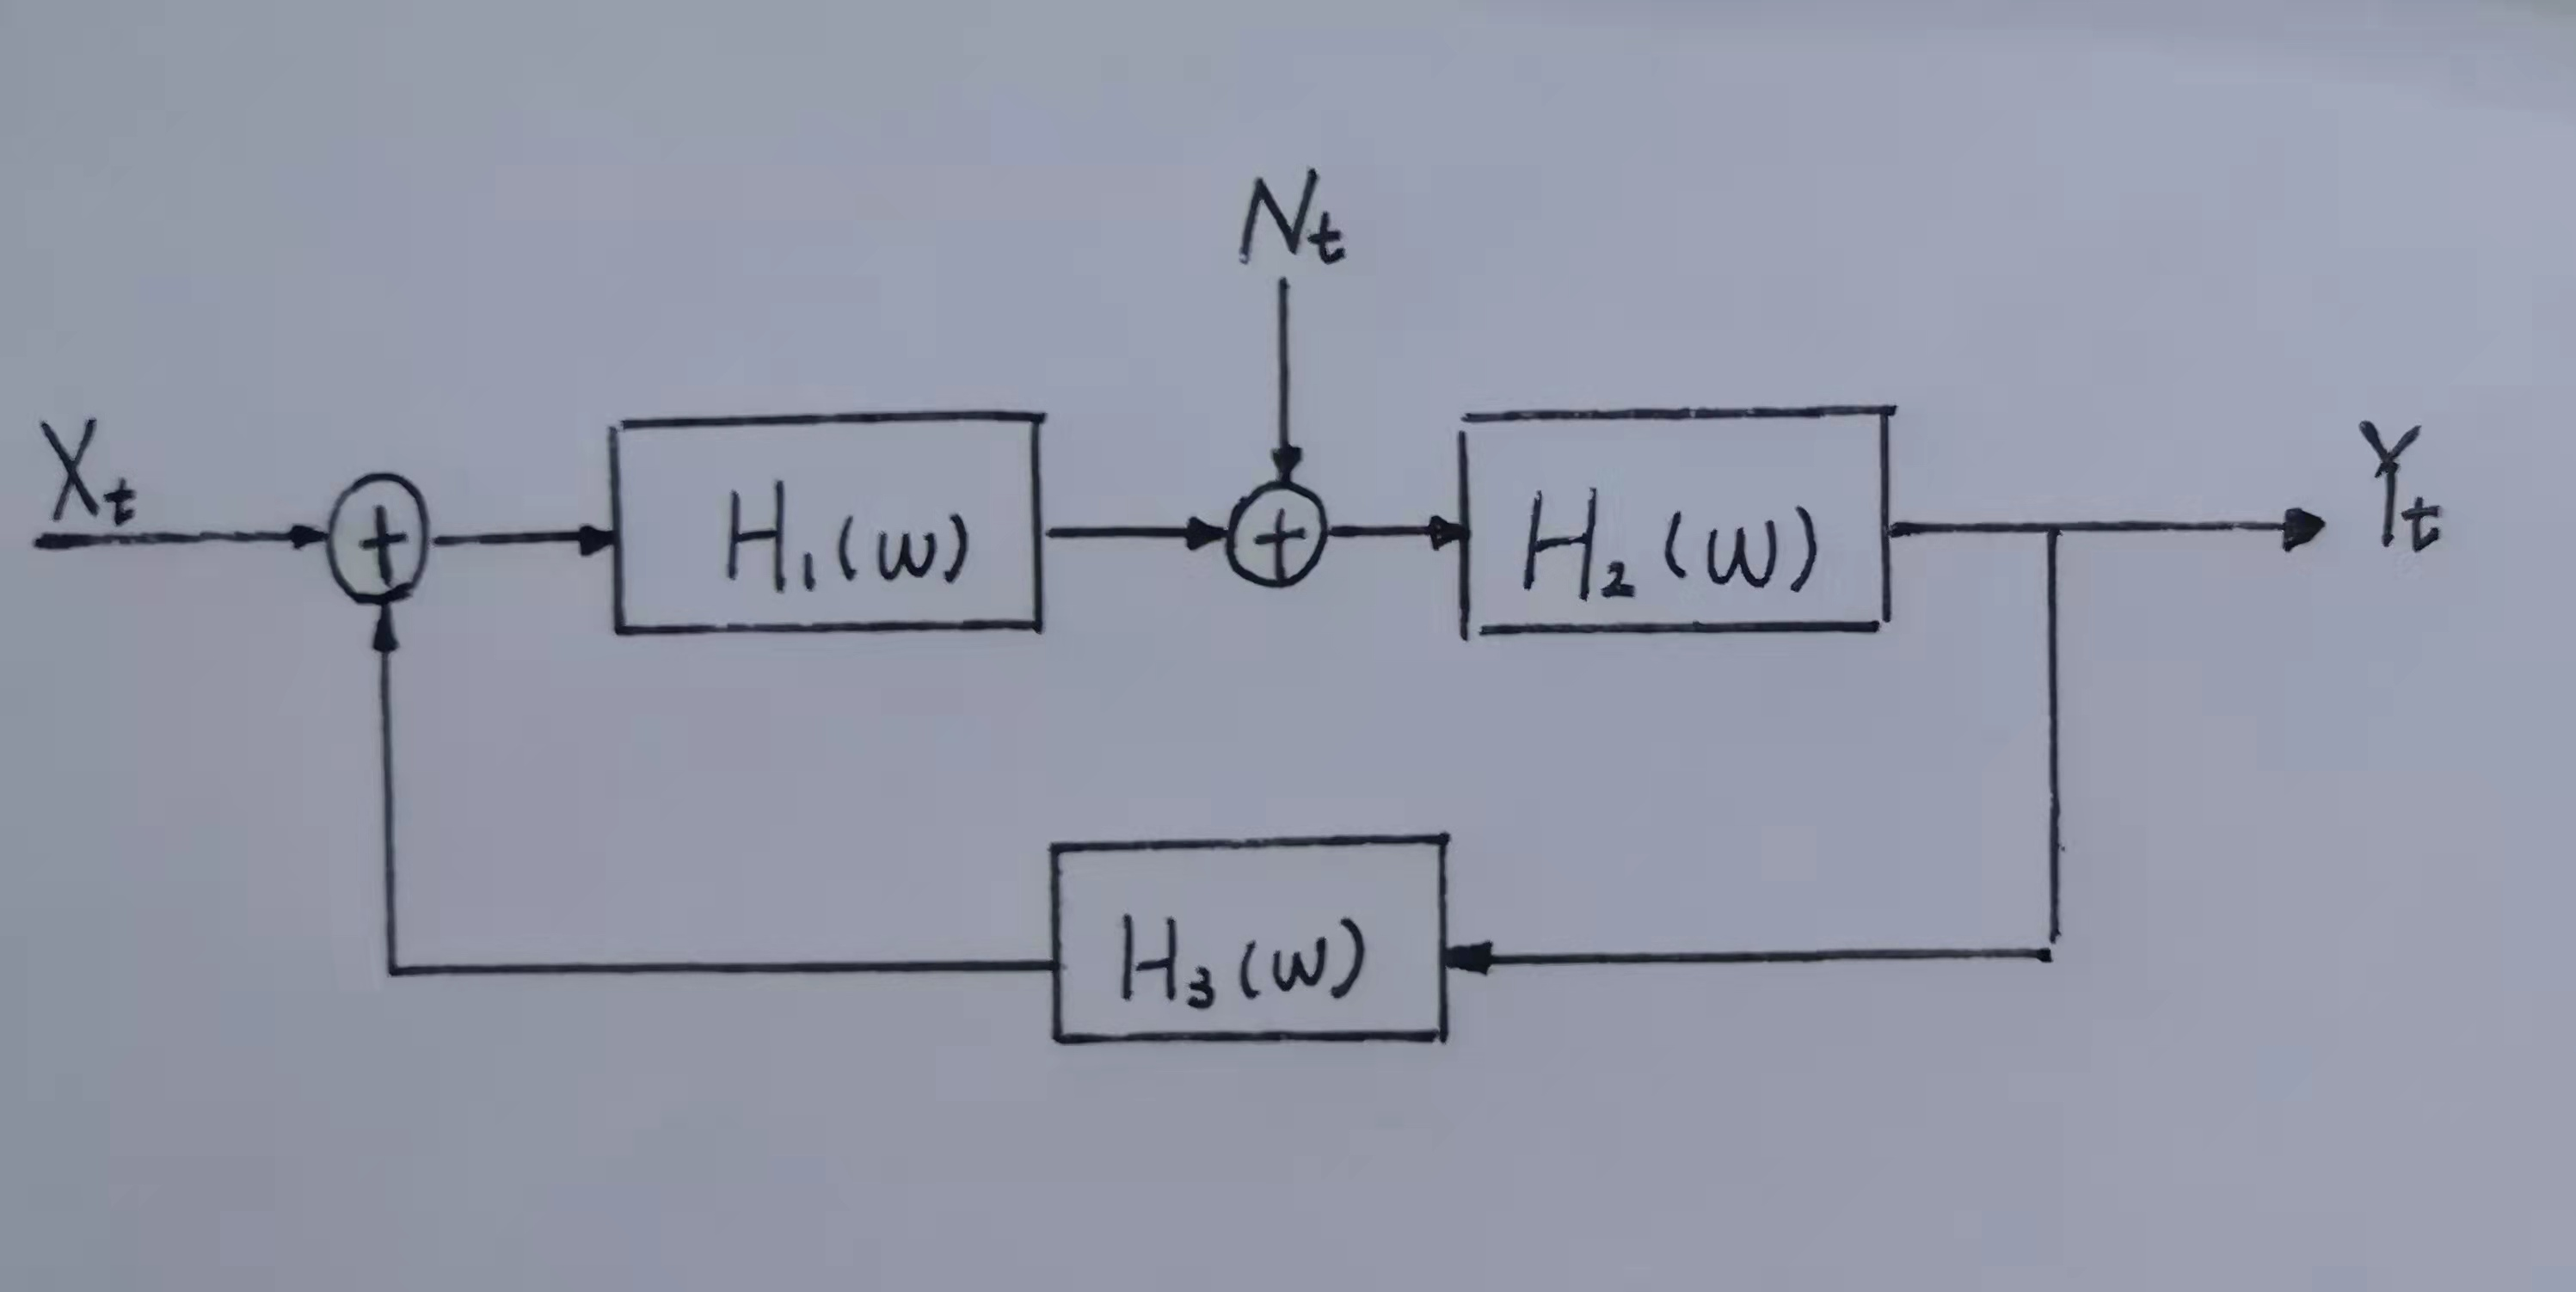
\includegraphics[width=8cm,height=3cm]{4.jpg}
\end{figure}
\begin{equation*}
  \begin{aligned}
     & Y(\omega)=((X(\omega)+H_3(\omega)Y(\omega))H_1(\omega)+N(\omega))H_2(\omega)
    =A(\omega)X(\omega)+B(\omega)Y(\omega)                                           \\
     & A(\omega)=\frac{H_2(\omega)H_1(\omega)}{1+H_1(\omega)H_2(\omega)H_3(\omega)},
    \quad B(\omega)=\frac{H_2(\omega)}{1+H_1(\omega)H_2(\omega)H_3(\omega)}          \\
     & S_Y(\omega)=\lvert A(\omega)\rvert^2S_X(\omega)+\lvert B(\omega)\rvert^2
    S_N(\omega)=\lvert A(\omega)\rvert^2S_X(\omega)+\lvert B(\omega)\rvert^2
    \frac{n_0}{2}                                                                    \\
  \end{aligned}
\end{equation*}
\section*{5.设X,Y为随机变量,设随机过程$Z(t)$满足$Z(t)=Xcos^2(t)+Ysin^2(t)$,请给出X,Y的
  具体例子,使得$Z(t)$分别为宽平稳和非宽平稳过程。}
\begin{equation*}
  \begin{aligned}
     & (1)Y=X,\quad X\sim U(0,1)      \\
     & (2)Y\equiv0,\quad X\sim U(0,1) \\
  \end{aligned}
\end{equation*}
\section*{6.设$U_n,n\in N$为独立同分布随机变量,服从$[0,1]$上的均匀分布,令$X_k=max(
    U_{k-1},U_k)$,计算随机过程$X_k$的相关函数。}
\begin{equation*}
  \begin{aligned}
     & X_k=max\{U_{k-1},U_k\},\quad F_X(x)=F_{U_1}(x)F_{U_2}(x)=x^2,\quad
    f_X(x)=2x,\quad E[X]=\frac{2}{3}                                      \\
     & (1)n\geq2,\quad R_X(n)=E[X_{m+n}]E[X_m]=\frac{4}{9}                \\
     & (2)n=0,\quad R_X(0)=E[X^2]=\frac{1}{2}                             \\
     & (3)n=1,\quad R_X(1)=E[X_nX_{n+1}]                                  \\
     & =\frac{1}{3}E[U_n^2\lvert U_n>U_{n-1},U_n>
    U_{n+1}]+\frac{1}{3}E[U_{n-1}U_{n+1}\lvert U_n<U_{n-1},U_n<U_{n+1}]   \\
     & +\frac{1}{6}E[U_{n-1}U_n\lvert U_{n-1}>U_n>U_{n+1}]
    +\frac{1}{6}E[U_{n+1}U_n\lvert U_{n+1}>U_n>U_{n-1}]                   \\
     & =\frac{1}{5}+\frac{4}{27}+\frac{1}{15}+\frac{1}{15}=\frac{13}{27}  \\
  \end{aligned}
\end{equation*}
\section*{7.设$N(t)$为Poission过程,参数为$\lambda$,请计算在时间段$[0,2]$内发生两次事
  件,且时间段$[1,3]$内发生两次事件的条件下,时间段$[1,2]$内发生事件次数的概率分布;并请计算
  在同样的条件下,时间段$[0,3]$内最早发生的事件和最晚发生的事件之间的时间间隔的均值。}
设$[0,1],[1,2],[2,3]$内发生事件的次数依次为$X_1,X_2,X_3$,事件从前到后依次为$Z_1,Z_2,
  \cdots$。题中描述的事件A为互斥事件$A_1,A_2,A_3$的并集。
\begin{equation*}
  \begin{aligned}
     & A_1:=\{X_1=X_3=2,X_2=0\},\quad A_2:=\{X_1=X_2=X_3=1\},\quad A_3:=\{X_1=
    X_3=0,X_2=2\}                                                                     \\
     & P(A_1)=\frac{\lambda^4}{4}e^{-3\lambda},\quad P(A_2)=\lambda^3e^{-3\lambda},
    \quad P(A_3)=\frac{\lambda^2}{2}e^{-3\lambda}                                     \\
     & P(A_1\lvert A)=\frac{\lambda^2}{\lambda^2+4\lambda+2},\quad
    P(A_2\lvert A)=\frac{4\lambda}{\lambda^2+4\lambda+2},\quad
    P(A_3\lvert A)=\frac{2}{\lambda^2+4\lambda+2}                                     \\
     & given\quad A_1,\quad F_{Z_1}(z)=2z-z^2,f_{Z_1}(z)=2-2z,E[Z_1]=\frac{1}{3}      \\
     & E[Z_2]=\frac{8}{3},E[Y\lvert A_1]=E[Z_4]-E[Z_1]=\frac{7}{3}                    \\
     & given\quad A_2,\quad Z_1\sim U(0,1),Z_3\sim U(2,3),E[Y\lvert A_2]=E[Z_3-Z_1]=2 \\
     & given\quad A_3, E[Y]=\frac{1}{\lambda}                                         \\
     & E[Y]=\frac{7\lambda^3+24\lambda^2+6}{3\lambda(\lambda^2+4\lambda+2)}
  \end{aligned}
\end{equation*}
\section*{8.设进入公园的人数服从参数为2的Poission流,每一个人在公园内停留的时间服从1小时
  到2小时之间的均匀分布,如果公园的初始人数为0,请计算公园内人数$N(t)$的均值和方差。}
设$X_k(t,\tau_k)=\begin{cases}
    1 \\
    0 \\
  \end{cases}$,$X_k=1$代表$\tau_k$时刻到达的人$t$时刻还在,反之为0。
\begin{equation*}
  \begin{aligned}
     & N(t)=\sum\limits_{k=1}^{Y(t)}X_k(t,\tau_k)                                        \\
     & E[X_k(t,\tau_k)]=\begin{cases}
      0,\quad t_k\geq t\quad or\quad\tau_k\leq t-2 \\
      1,\quad t-1\leq\tau_k<t                      \\
      2-t+\tau_k,\quad t-2<\tau_k<t-1              \\
    \end{cases}                                       \\
     & E[X^2]=E[X]                                                                       \\
     & given\quad t\geq2,\quad\int_0^t E[X(t,\tau)]d\tau=\int_{t-2}^{t-1}(2-t+\tau)d\tau
    +\int_{t-1}^td\tau=\frac{3}{2}                                                       \\
     & \therefore E[Y(t)]=\lambda\int_0^t E[X(t,\tau)]d\tau=
    \begin{cases}
      2t,\quad0\leq t\leq1 \\
      -t^2+4t-3,\quad1<t<2 \\
      3,\quad t\geq2       \\
    \end{cases}                                                           \\
     & Var[Y(t)]=\lambda\int_0^t E[X^2(t,\tau)]d\tau=
    \begin{cases}
      2t,\quad0\leq t\leq1 \\
      -t^2+4t-3,\quad1<t<2 \\
      3,\quad t\geq2       \\
    \end{cases}                                                           \\
  \end{aligned}
\end{equation*}
\section*{9.考虑正立方体,一只蚂蚁在该立方体上运动,每一步都从一个顶点到与之相邻的三个顶
  点之一。设蚂蚁到达三个顶点的概率相同。设蚂蚁的起点为顶点a,$Y_n$为蚂蚁第n不到达的顶点与a点
  之间的最短距离,请给出Markov链$Y_n$的一步转移概率矩阵,并计算其极限分布。}
\begin{equation*}
  \begin{aligned}
     & Y_n=\{0,1,\sqrt2,\sqrt3\},P=\begin{bmatrix}
      0           & 1           & 0           & 0           \\
      \frac{1}{3} & 0           & \frac{2}{3} & 0           \\
      0           & \frac{2}{3} & 0           & \frac{1}{3} \\
      0           & 0           & 1           & 0           \\
    \end{bmatrix},
    \pi=\pi\cdot P,\pi_0=\pi_3=\frac{1}{8},\pi_1=\pi_2=\frac{3}{8}
  \end{aligned}
\end{equation*}
\section*{10.考虑三个不可分辨的球,分别放在数轴的整数点上,每个点上允许放置不止一个球。球的
  位置按照如下步骤进行变动,每一步的具体做法是:将最左端的球拿起,从剩下两个球中等概率地选取一
  个(不拿起),将拿起的球放置到选中的球所在整数点的右侧相邻整数点上。请构造Markov链来描述三个
  球的相对位置关系,写出一步转移概率矩阵,并计算其极限概率分布。}
考虑以下简化方法:定义左、中两球间距为$n$,中、右两球间距为$m$的状态为$(m,n)$,则所有的状态
可以被归结为5种:$(m,n),(m,1),(1,1),(1,0),(0,1)$,其状态转移矩阵为
\begin{equation*}
  \begin{aligned}
     & P=\begin{bmatrix}
      \frac{1}{2} & \frac{1}{2} & 0           & 0           & 0 \\
      0           & 0           & \frac{1}{2} & \frac{1}{2} & 0 \\
      0           & 0           & \frac{1}{2} & \frac{1}{2} & 0 \\
      0           & 0           & 0           & 0           & 1 \\
      0           & 0           & \frac{1}{2} & \frac{1}{2} & 0 \\
    \end{bmatrix},
    \pi=\pi\cdot P,\pi_1=\pi_2=0,\pi_3=\pi_4=\pi_5=\frac{1}{3} \\
  \end{aligned}
\end{equation*}

\end{document}